% !TEX TS-program = XeLaTeX
\documentclass[a4paper]{article}
\usepackage{tikz}

% https://tex.stackexchange.com/questions/172234/define-and-set-length-in-one-command
\newcommand{\deflen}[2]{%      
    \expandafter\newlength\csname #1\endcsname
    \expandafter\setlength\csname #1\endcsname{#2}%
}

\newcommand{\goldenratio}{1.618}

\deflen{horizontalmarg}{1.0cm}
\deflen{verticalmarg}{\dimexpr(\goldenratio\horizontalmarg)}

\usepackage[top=\the\verticalmarg, bottom=\the\verticalmarg, 
  left=\the\horizontalmarg, right=\the\horizontalmarg]{geometry}


\deflen{lowerbaroffset}{0.8cm}


\newlength{\localpwidth}

\deflen{contentswidth}{\dimexpr(\paperwidth-2\horizontalmarg)}
\deflen{contentsheight}{\dimexpr(\paperheight-2.01\verticalmarg)}

\deflen{halfwidth}{\dimexpr(0.5\contentswidth)}


\deflen{paramarg}{0.5cm}

\deflen{colwidth}{\dimexpr(\halfwidth-\paramarg)}

\deflen{lowersectionstart}{\dimexpr(0.5\contentsheight)}
\deflen{headermarg}{2cm}

%% The vertical lines at which things should align
\deflen{haligni}{0cm}
\deflen{halignii}{\colwidth}
\deflen{haligniii}{\dimexpr(\halfwidth+\paramarg)}
\deflen{haligniv}{\dimexpr(\contentswidth)}

\deflen{valigni}{\contentsheight}
\deflen{valignii}{\dimexpr(\contentsheight-\headermarg)}
\deflen{valigniii}{\lowersectionstart}
\deflen{valigniv}{\dimexpr(\lowersectionstart-\headermarg)}

\usepackage{fontspec,lipsum}


% Draw a vertical bar across the contents area
\newcommand{\vhelper}[1]{\draw[color=gray] (#1,0cm) -- (#1,\the\contentsheight);}

% Draw a horizontal bar across the contents area
\newcommand{\hhelper}[1]{\draw[color=gray] (0cm,#1) -- (\the\contentswidth,#1);}

% Display helper lines
\newcommand{\helpers}{
  \draw[color=gray] (0,0) rectangle (\the\contentswidth, \the\contentsheight);
  \vhelper{\the\halignii}
  \vhelper{\the\haligniii}
  \hhelper{\the\valignii}
  \hhelper{\the\valigniii}
  \hhelper{\the\valigniv}
}

% A4: 21.0 × 29.7
\pagenumbering{gobble}
\setmainfont[Path=../fonts/]{Muli-Regular.ttf}


% (x, y, pos)
\newcommand{\mainheader}[3]{
  \setmainfont[Path=../fonts/]{BoingBold.otf}
  \node[anchor=north west] at (#1,#2) {\Huge #3};
  \setmainfont[Path=../fonts/]{Muli-Regular.ttf}
}



% TODO: See if Melissa provided some design document
% with precise specs of margins, font sizes, etc.

\begin{document}
\noindent
\begin{tikzpicture}[x=1cm, y=1cm]
\definecolor{anemored}{rgb} {1.00,0.129,0.247}
\helpers

\mainheader{\the\haligni}{\the\valigni}{anemobox specs}

% Right column
\node[anchor=north west] at (\the\haligniii,\the\valignii) {
  \begin{minipage}[l]{\the\colwidth}
    This is really great!
  \end{minipage}
};

\mainheader{\the\haligni}{\the\valigniii}{anemobox order form}

%\node[inner sep=0pt, anchor=north west] (anemobox) at (0cm,\the\contentsheight) {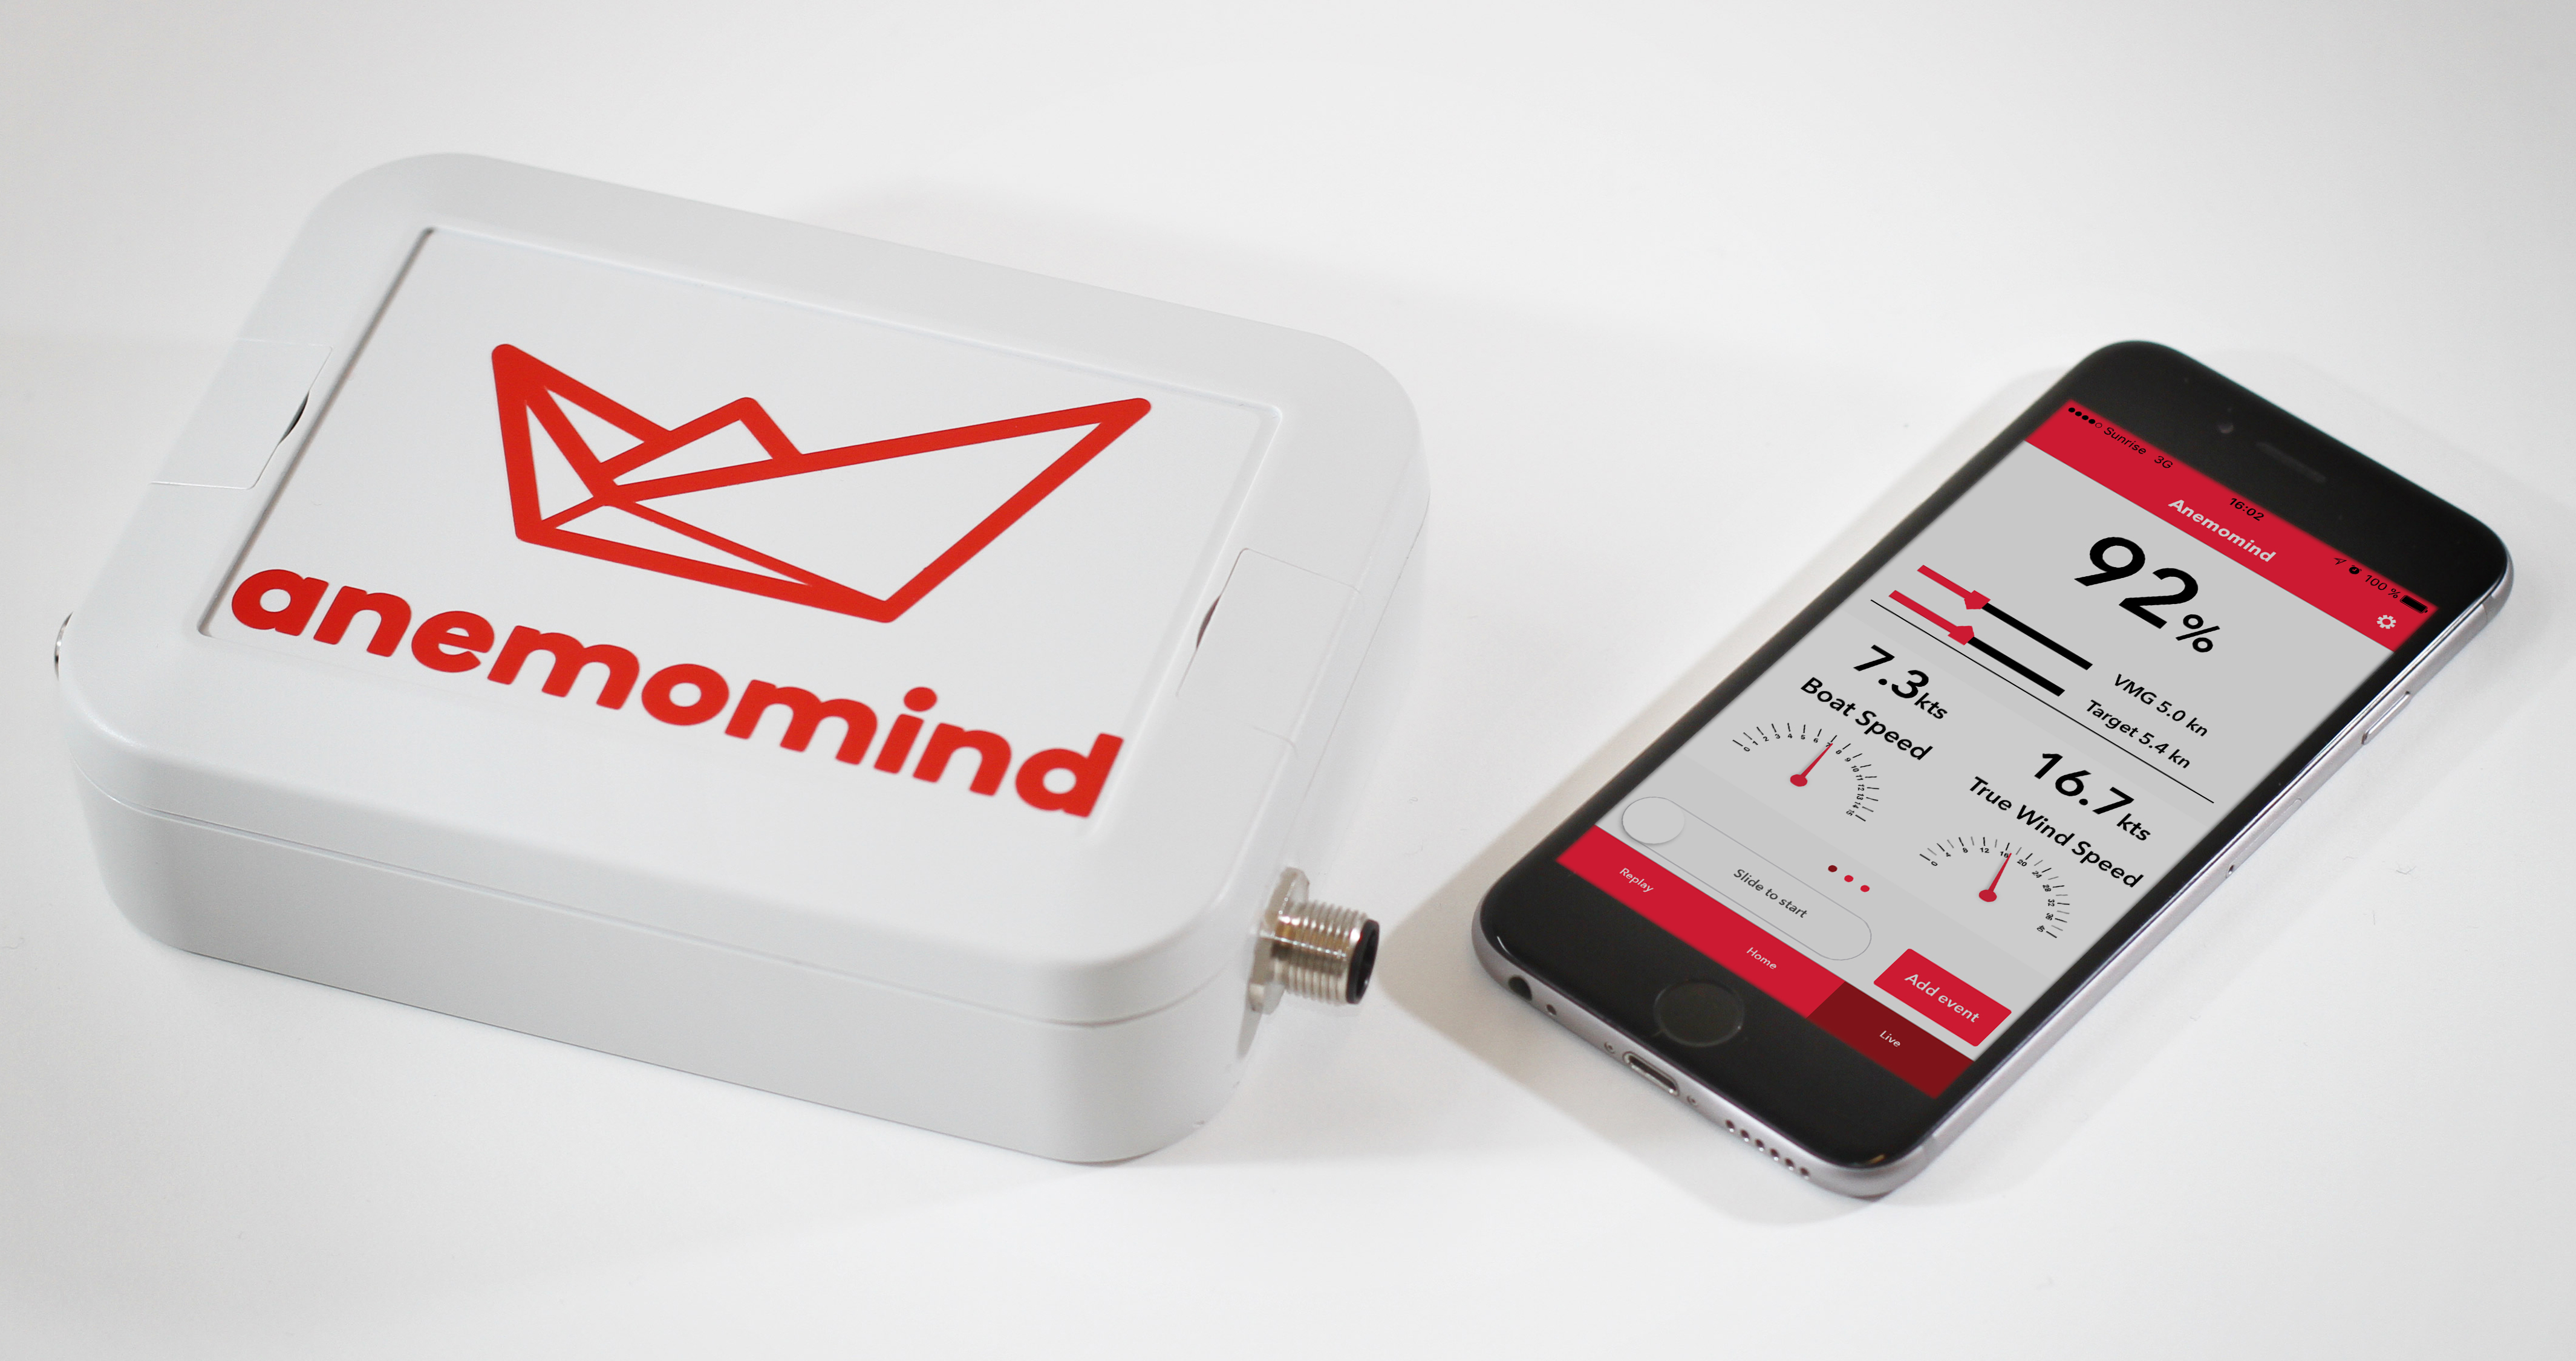
\includegraphics[width=\the\halfwidth]{../images/anemobox10.jpg}};

%% \foreach \bound in {north,south,west,east,45} {
%%       \node[anchor=\bound] at (current page.\bound) {I am \bound-bound...};
%%   }
  \node[anchor=north west, color=anemored] at (0, \the\contentsheight) {\Large Specifications!};
  \draw[color=anemored, line width=0.25mm] (0, \the\dimexpr(\contentsheight-\lowerbaroffset)) -- (\the\localpwidth, \the\dimexpr(\contentsheight-\lowerbaroffset));
%\node[draw=none] at (0,0) {some text};
%\node[draw] at (0,0) {some text};

\end{tikzpicture}
\end{document} 

